\documentclass{article}
\usepackage{listings}
\usepackage{xcolor}
\usepackage{graphicx}
\usepackage{caption}
\usepackage{amsmath}

\definecolor{codeblue}{rgb}{0.1,0.1,0.6}
\definecolor{backgrey}{rgb}{0.95,0.95,0.95}

\lstset{
  backgroundcolor=\color{backgrey},
  basicstyle=\ttfamily\footnotesize,
  keywordstyle=\color{codeblue}\bfseries,
  commentstyle=\color{gray}\itshape,
  stringstyle=\color{orange},
  showstringspaces=false,
  breaklines=true,
  frame=single,
  postbreak=\mbox{\textcolor{red}{$\hookrightarrow$}\space},
  numbers=left,
  numberstyle=\tiny\color{gray}
}

\begin{document}

\section*{Image Preprocessing and Binary Conversion}

The following Python code demonstrates how to:
\begin{enumerate}
    \item Download and extract image data.
    \item Convert the image into a binary format using pixel intensity thresholding.
    \item Modify the image visually using the Pillow library.
\end{enumerate}

\subsection*{Code}

\begin{lstlisting}[language=Python]
# Install gdown and download ZIP file
!pip install --upgrade --no-cache-dir gdown
!gdown 1QTi7dJtNAfFR5mG0rd8K3ZGvEIfSn_DS
!unzip PersianData.zip

import numpy as np
from PIL import Image, ImageDraw
import random
import os
import matplotlib.pyplot as plt

def convertImageToBinary(path):
    """
    Convert an image to a binary representation based on pixel intensity.

    Args:
        path (str): The file path to the input image.

    Returns:
        list: A binary representation of the image where white is represented by -1 
              and black is represented by 1.
    """
    image = Image.open(path)
    draw = ImageDraw.Draw(image)
    width, height = image.size
    pix = image.load()
    factor = 100
    binary_representation = []

    for i in range(width):
        for j in range(height):
            red, green, blue = pix[i, j][:3]
            total_intensity = red + green + blue

            if total_intensity > (((255 + factor) // 2) * 3):
                red, green, blue = 255, 255, 255
                binary_representation.append(-1)
            else:
                red, green, blue = 0, 0, 0
                binary_representation.append(1)

            draw.point((i, j), (red, green, blue))

    del draw
    return binary_representation
\end{lstlisting}

\subsection*{Explanation}
\begin{itemize}
    \item \textbf{Lines 1-3:} Install `gdown`, download the ZIP archive from Google Drive, and extract it.
    \item \textbf{Lines 5-10:} Import required libraries for image handling, math, and plotting.
    \item \textbf{Function \texttt{convertImageToBinary}:}
    \begin{itemize}
        \item Opens an image using PIL.
        \item Reads each pixel's RGB values.
        \item Calculates intensity as sum of RGB.
        \item Uses a threshold value to binarize the image.
        \item Changes image pixels to white (RGB: 255,255,255, encoded as -1) or black (RGB: 0,0,0, encoded as 1).
        \item Modifies the image directly and returns a flattened list of binary values.
    \end{itemize}
\end{itemize}



\documentclass{article}
\usepackage{listings}
\usepackage{xcolor}
\usepackage{tcolorbox}
\usepackage{amsmath}

\definecolor{codeblue}{rgb}{0,0,0.5}
\definecolor{backgray}{rgb}{0.96,0.96,0.96}
\definecolor{commentgray}{rgb}{0.4, 0.4, 0.4}

\lstset{
  backgroundcolor=\color{backgray},
  basicstyle=\ttfamily\small,
  keywordstyle=\color{codeblue}\bfseries,
  commentstyle=\color{commentgray}\itshape,
  stringstyle=\color{orange},
  showstringspaces=false,
  breaklines=true,
  frame=single,
  numbers=left,
  numberstyle=\tiny\color{gray},
  captionpos=b
}

\begin{document}

\section*{Generating Noisy Images in Python}

The following Python code creates noisy versions of a set of image files by adding random noise to each pixel’s RGB values. The processed images are then saved under new filenames.

\subsection*{Python Code}

\begin{lstlisting}[language=Python, caption={Code to generate noisy images from original image files.}]
from PIL import Image, ImageDraw
import random

def generateNoisyImages():
    # List of image file paths
    image_paths = [
        "/content/1.jpg",
        "/content/2.jpg",
        "/content/3.jpg",
        "/content/4.jpg",
        "/content/5.jpg"
    ]

    for i, image_path in enumerate(image_paths, start=1):
        noisy_image_path = f"/content/noisy{i}.jpg"
        getNoisyBinaryImage(image_path, noisy_image_path)
        print(f"Noisy image for {image_path} generated and saved as {noisy_image_path}")

def getNoisyBinaryImage(input_path, output_path):
    """
    Add noise to an image and save it as a new file.

    Args:
        input_path (str): The file path to the input image.
        output_path (str): The file path to save the noisy image.
    """
    # Open the input image.
    image = Image.open(input_path)

    # Create a drawing tool for manipulating the image.
    draw = ImageDraw.Draw(image)

    # Determine the image's width and height in pixels.
    width = image.size[0]
    height = image.size[1]

    # Load pixel values for the image.
    pix = image.load()

    # Define a factor for introducing noise.
    noise_factor = 10000000

    # Loop through all pixels in the image.
    for i in range(width):
        for j in range(height):
            # Generate a random noise value within the specified factor.
            rand = random.randint(-noise_factor, noise_factor)

            # Add the noise to the Red, Green, and Blue (RGB) values of the pixel.
            red = pix[i, j][0] + rand
            green = pix[i, j][1] + rand
            blue = pix[i, j][2] + rand

            # Ensure that RGB values stay within the valid range (0-255).
            if red < 0:
                red = 0
            if green < 0:
                green = 0
            if blue < 0:
                blue = 0
            if red > 255:
                red = 255
            if green > 255:
                green = 255
            if blue > 255:
                blue = 255

            # Set the pixel color accordingly.
            draw.point((i, j), (red, green, blue))

    # Save the noisy image as a file.
    image.save(output_path, "JPEG")

    # Clean up the drawing tool.
    del draw
\end{lstlisting}

\subsection*{Explanation}

\begin{tcolorbox}[colback=white, colframe=black, title=Function: \texttt{generateNoisyImages}]
This function initializes a list of 5 image paths (e.g., 1.jpg to 5.jpg). It loops through them using \texttt{enumerate}, and for each image:
\begin{itemize}
  \item Calls \texttt{getNoisyBinaryImage()} to generate a noisy version
  \item Saves the new image with the prefix \texttt{noisy\#.jpg}
\end{itemize}
\end{tcolorbox}

\begin{tcolorbox}[colback=white, colframe=black, title=Function: \texttt{getNoisyBinaryImage}]
This function applies pixel-wise noise to an image:
\begin{enumerate}
    \item Loads the image using \texttt{PIL.Image}.
    \item Accesses pixel data and creates a \texttt{Draw} object to edit it.
    \item For every pixel:
    \begin{itemize}
        \item Adds a random value (from \texttt{-noise\_factor} to \texttt{+noise\_factor}) to each of the R, G, and B channels.
        \item Clips values to the valid range [0, 255].
        \item Sets the modified color to the pixel.
    \end{itemize}
    \item Saves the modified image to the output path.
\end{enumerate}
Note: The current \texttt{noise\_factor = 10000000} is very high and will turn most pixels fully black or white. Use values like 30--50 for realistic noise.
\end{tcolorbox}

\subsection*{Integration Note}

This code is self-contained and can be safely appended to an existing image processing project. Ensure that `PIL` and `random` are already imported in your main script.


\section*{1. Function: \texttt{convertImageToBinary}}

\begin{lstlisting}[language=Python, caption={Convert image to binary array based on intensity}]
def convertImageToBinary(path: str, factor: int=100, output_path : str = None):
    """
    Convert an image to a binary representation based on pixel intensity.
    Args:
        path (str): The file path to the input image.
        factor (int, optional): Adjusts the binarization threshold (Default: 100).
    Returns:
        list: A binary representation of the image where white is -1 and black is 1.
    """
    with Image.open(path) as img:
        image = img.convert("RGB")

    img_array = np.array(image)
    intensity = img_array.sum(axis=2)
    threshold = ((255 + factor) // 2) * 3
    binary_representation = np.where(intensity > threshold, -1, 1).flatten()

    if output_path:
        binarized_array = np.where(intensity > threshold, 255, 0)
        binarized_array = np.stack([binarized_array]*3, axis=-1)
        binarized_image = Image.fromarray(binarized_array.astype("uint8"), "RGB")
        binarized_image.save(output_path, 'JPEG')
    
    return binary_representation
\end{lstlisting}

\begin{tcolorbox}[colback=white, colframe=black, title=Explanation: \texttt{convertImageToBinary}]
This function reads an RGB image and converts it into a binary 1D array, based on the total intensity of each pixel.
\begin{itemize}
  \item Converts the image to a NumPy array and calculates total brightness by summing R, G, and B values.
  \item Compares the summed intensity to a threshold determined by \texttt{factor}.
  \item Returns \texttt{-1} for bright pixels and \texttt{1} for dark ones.
  \item If an \texttt{output\_path} is given, it also saves the visual binarized image with only black and white values.
\end{itemize}
\end{tcolorbox}


\section*{2. Function: \texttt{getNoisyBinaryImage}}

\begin{lstlisting}[language=Python, caption={Add noise to an image and save it}]
def getNoisyBinaryImage(input_path, output_path, noise_factor=10000000, random_state=None):
    """
    Add noise to an image and save it as a new file.
    Args:
        input_path (str): Input image path.
        output_path (str): Output image save path.
        noise_factor (int): Amplitude of noise (default: 10,000,000).
        random_state (int/None): Seed for reproducibility.
    """
    with Image.open(input_path) as img:
        image = img.convert("RGB")

    img_array = np.array(image)

    if random_state is not None:
        np.random.seed(random_state)

    rand = np.random.randint(-noise_factor, noise_factor, img.size[0:2])
    
    red   = np.clip(img_array[:, :, 0] + rand, 0, 255)
    green = np.clip(img_array[:, :, 1] + rand, 0, 255)
    blue  = np.clip(img_array[:, :, 2] + rand, 0, 255)

    noise_image = np.stack((red, green, blue), axis=2)
    noise_image = Image.fromarray(noise_image.astype("uint8"), "RGB")
    noise_image.save(output_path, "JPEG")
\end{lstlisting}

\begin{tcolorbox}[colback=white, colframe=black, title=Explanation: \texttt{getNoisyBinaryImage}]
This function injects pixel-wise random noise to the RGB channels of an image:
\begin{itemize}
  \item Noise is generated in the range of \texttt{[-noise\_factor, +noise\_factor]}.
  \item The same noise value is added to all 3 channels (R, G, B).
  \item Uses \texttt{np.clip} to keep values within [0, 255].
  \item Optionally seeds the random generator for reproducible results.
  \item Saves the resulting image to disk.
\end{itemize}
\end{tcolorbox}


\section*{3. Function: \texttt{generateNoisyImages}}

\begin{lstlisting}[language=Python, caption={Batch generation of noisy images}]
def generateNoisyImages(noise_factor=10000000, random_state = None):
    # List of image file paths
    image_paths = [
        "1.jpg", "2.jpg", "3.jpg", "4.jpg", "5.jpg"
    ]

    os.makedirs('noisy', exist_ok=True)
    for i, image_path in enumerate(image_paths, start=1):
        noisy_image_path = f"noisy/noisy{i}.jpg"
        getNoisyBinaryImage(image_path, noisy_image_path, noise_factor, random_state)
        print(f"Noisy image for {image_path} generated and saved as {noisy_image_path}")
\end{lstlisting}

\begin{tcolorbox}[colback=white, colframe=black, title=Explanation: \texttt{generateNoisyImages}]
This utility function processes a batch of 5 predefined images:
\begin{itemize}
  \item Calls \texttt{getNoisyBinaryImage} for each image.
  \item Stores outputs in a folder named \texttt{noisy}.
  \item Useful for automated dataset augmentation.
\end{itemize}
\end{tcolorbox}


\section*{4. Function: \texttt{BinarytoImage}}

\begin{lstlisting}[language=Python, caption={Convert a binary array back to an image}]
def BinarytoImage(binary_img):
    binary_img = np.array(binary_img)
    img = np.where(binary_img == -1, 255, 0)
    img = img.reshape(96,96)
    img = np.stack([img]*3, axis=2)
    img = Image.fromarray(img.astype("uint8"), "RGB")
    return img
\end{lstlisting}

\begin{tcolorbox}[colback=white, colframe=black, title=Explanation: \texttt{BinarytoImage}]
This function reconstructs a 96x96 RGB image from a binary array:
\begin{itemize}
  \item Pixels with value \texttt{-1} are set to white (255).
  \item Pixels with value \texttt{1} are set to black (0).
  \item Expands single-channel grayscale into 3-channel RGB.
  \item Returns the image (but does not save it).
\end{itemize}
\end{tcolorbox}


\section*{5. Class: \texttt{HammingNetwork}}

\begin{lstlisting}[language=Python, caption={Define and use a Hamming network for pattern classification}]
class HammingNetwork:
    def __init__(self, patterns):
        self.patterns = np.array([p for p in patterns])
        self.n_classes = len(patterns)

    def predict(self, x_noisy):
        similarities = np.dot(self.patterns, x_noisy)
        return self.patterns[np.argmax(similarities)]

# Load training patterns (binary vectors) from 5 clean images
images = [convertImageToBinary(f'{i}.jpg') for i in range(1, 6)]
model = HammingNetwork(images)
\end{lstlisting}

\begin{tcolorbox}[colback=white, colframe=black, title=Explanation: \texttt{HammingNetwork}]
This class implements a Hamming network for pattern recognition based on similarity (dot product) between binary vectors:
\begin{itemize}
  \item \texttt{\_\_init\_\_} stores the input patterns and calculates the number of classes.
  \item \texttt{predict()} computes the dot product (similarity) between the noisy input and all stored patterns, then returns the most similar one.
  \item In the example, the model is trained using binarized versions of five clean images.
\end{itemize}
\end{tcolorbox}


\section*{6. Generate Noisy Images and Convert to Binary}

\begin{lstlisting}[language=Python, caption={Generate noisy images and convert them to binary vectors}]
generateNoisyImages(1100, 93)
paths = [f'noisy/noisy{i}.jpg' for i in range(1, 6)]
noise = [convertImageToBinary(f'{i}') for i in paths]
\end{lstlisting}

\begin{tcolorbox}[colback=white, colframe=black, title=Explanation: Noisy Image Processing]
\begin{itemize}
  \item Noisy versions of the 5 training images are generated using \texttt{generateNoisyImages()}.
  \item Each noisy image is then converted into a binary vector using \texttt{convertImageToBinary()}.
  \item These binary vectors simulate noisy inputs to be classified by the Hamming network.
\end{itemize}
\end{tcolorbox}


\section*{7. Visualization and Prediction}

\begin{lstlisting}[language=Python, caption={Visualize noisy images and their Hamming predictions}]
def show_images(noise, predictions):
    fig, axes = plt.subplots(2, 5, figsize=(15, 5))
    for i in range(5):
        n = noise[i]
        p = predictions[i]
        axes[0, i].imshow(n, cmap='gray')
        axes[0, i].set_title(f"Noisy {i+1}")
        axes[0, i].axis('off')

        axes[1, i].imshow(p, cmap='gray')
        axes[1, i].set_title(f"Prediction {i+1}")
        axes[1, i].axis('off')

    plt.tight_layout()
    plt.show()

# Predict the class for each noisy binary input
per = [model.predict(noise[i]) for i in range(5)]

# Convert binary arrays back to images
noise_img = [BinarytoImage(noise[i]) for i in range(5)]
per_img = [BinarytoImage(per[i]) for i in range(5)]

# Display the noisy and predicted images side by side
show_images(noise_img, per_img)
\end{lstlisting}

\begin{tcolorbox}[colback=white, colframe=black, title=Explanation: Prediction and Display]
\begin{itemize}
  \item The \texttt{show\_images()} function displays noisy and predicted images in a 2-row grid.
  \item The predictions are generated by the trained \texttt{HammingNetwork}.
  \item Both input noise and predicted output are converted from binary vectors back to RGB images using \texttt{BinarytoImage()}.
  \item This visual comparison is helpful to evaluate the robustness of the Hamming network under noise.
\end{itemize}
\end{tcolorbox}


\begin{figure}[h]
    \centering
    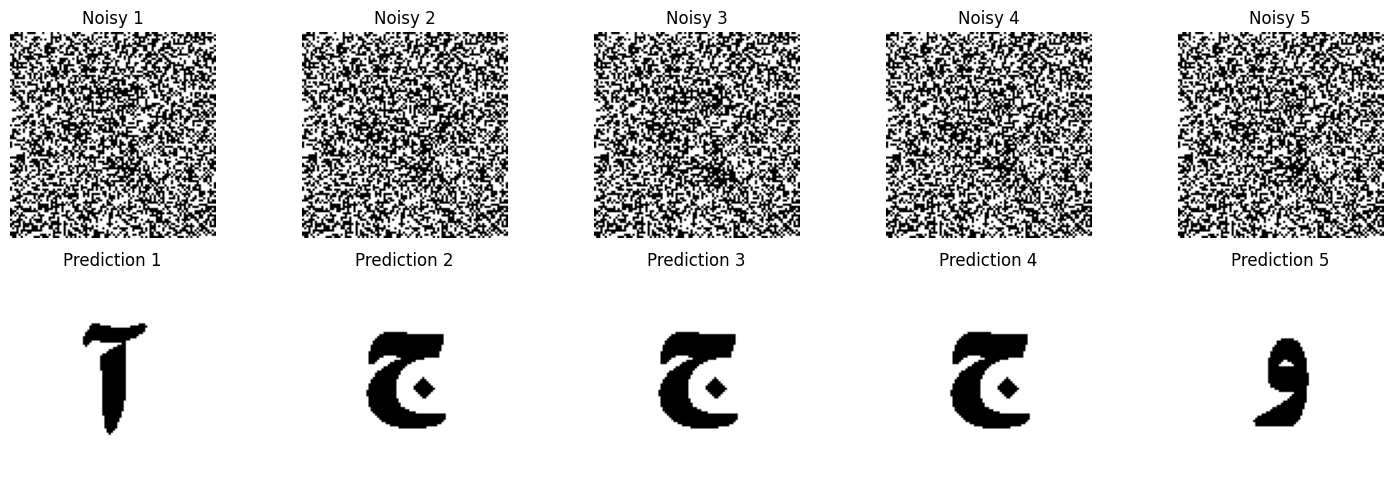
\includegraphics[width=0.5\textwidth]{3.png}
    \caption{Caption describing the image.}
    \label{fig:example}
\end{figure}



\section*{8. Functions: \texttt{missimage} and \texttt{generatemissimage}}

\begin{lstlisting}[language=Python, caption={Create synthetic missing-data images by whitening black pixels}]
def missimage(input_path, output_path, percent=20, factor=100, random_state=None):
    with Image.open(input_path) as img:
        image = img.convert("RGB")

    img_array = np.array(image)
    intensity = img_array.sum(axis=2)
    threshold = ((255 + factor) // 2) * 3
    blackpix = np.where(intensity < threshold)
    number = round(len(blackpix[0]) * percent / 100)

    if random_state is not None:
        np.random.seed(random_state)

    pixels_to_flip = np.random.choice(range(len(blackpix[0])), size=number, replace=False)
    img_array[blackpix[0][pixels_to_flip], blackpix[1][pixels_to_flip]] = 255
    img = Image.fromarray(img_array.astype("uint8"), "RGB")
    img.save(output_path, "JPEG")

def generatemissimage(percent=20, factor=100, random_state=None):
    image_paths = ["1.jpg", "2.jpg", "3.jpg", "4.jpg", "5.jpg"]
    os.makedirs('miss', exist_ok=True)
    for i, image_path in enumerate(image_paths, start=1):
        miss_image_path = f"miss/miss{i}.jpg"
        missimage(image_path, miss_image_path, percent, factor, random_state)
        print(f"Miss image for {image_path} generated and saved as {miss_image_path}")
\end{lstlisting}

\begin{tcolorbox}[colback=white, colframe=black, title=Explanation: \texttt{missimage}]
This function simulates partial data loss in images by randomly selecting a percentage of black pixels and converting them to white:
\begin{itemize}
  \item Pixel intensity is calculated to identify black pixels.
  \item A random subset of these pixels is turned white.
  \item The result is saved as a new image file.
\end{itemize}
The \texttt{generatemissimage} function applies this corruption to five original images and stores them in a \texttt{miss/} directory.
\end{tcolorbox}


\section*{9. Prediction and Visualization for Missed Images}

\begin{lstlisting}[language=Python, caption={Convert missed images to binary, predict using Hamming, and visualize}]
generatemissimage(70, 100, 93)
paths = [f'miss/miss{i}.jpg' for i in range(1, 6)]
miss = [convertImageToBinary(i) for i in paths]

per = [model.predict(miss[i]) for i in range(5)]
miss_img = [BinarytoImage(miss[i]) for i in range(5)]
per_img = [BinarytoImage(per[i]) for i in range(5)]
show_images(miss_img, per_img)
\end{lstlisting}

\begin{tcolorbox}[colback=white, colframe=black, title=Explanation: Evaluation on Missed Data]
\begin{itemize}
  \item Corrupted "miss" images are loaded and binarized.
  \item The Hamming network predicts which original pattern each corrupted image most closely matches.
  \item The \texttt{show\_images} function displays the corrupted (input) and predicted (output) images for comparison.
\end{itemize}
This test shows the model’s robustness to partial loss of pixel data (e.g., occlusion or dropout).
\end{tcolorbox}


\section*{10. Visual Output of Prediction on Missed Images}

\begin{figure}[h]
    \centering
    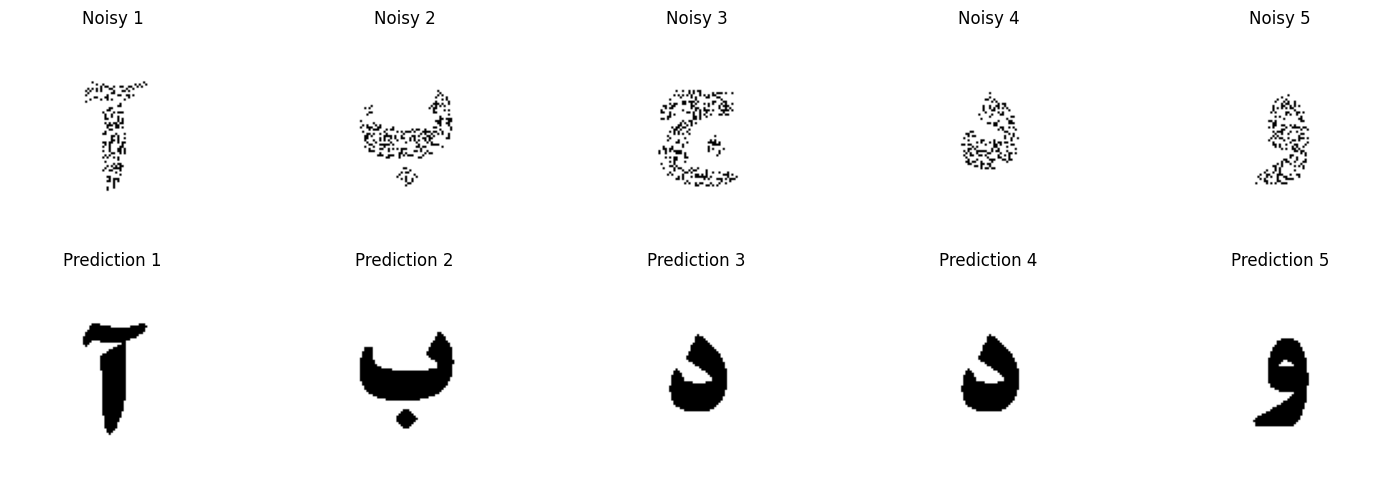
\includegraphics[width=\textwidth]{4.png}
    \caption{Top row: Partially erased (70\%) images. Bottom row: Predictions made by the Hamming network.}
    \label{fig:missed_predictions}
\end{figure}

\section*{11. Updated Class: \texttt{HammingNetwork} with Masking for Missing Pixels}

\begin{lstlisting}[language=Python, caption={Updated Hamming network that ignores missing (-1) pixels}]
class HammingNetwork:
    def __init__(self, patterns):
        self.patterns = np.array([p for p in patterns])
        self.n_classes = len(patterns)

    def masked_dot(self, a, b, mask):
        return np.dot(a[mask], b[mask])

    def predict(self, x_noisy):
        mask = x_noisy != -1
        similarities = [self.masked_dot(p, x_noisy, mask) for p in self.patterns]
        return self.patterns[np.argmax(similarities)]

# Initialize updated model
model = HammingNetwork(images)
\end{lstlisting}

\begin{tcolorbox}[colback=white, colframe=black, title=Explanation: \texttt{HammingNetwork} with Missing Pixel Handling]
This version improves upon the previous Hamming network by accounting for missing data in the input:
\begin{itemize}
  \item The input vector \texttt{x\_noisy} may contain \texttt{-1} values indicating missing pixels.
  \item A boolean mask is created to identify which elements are valid (not -1).
  \item The dot product is computed only over the valid (unmasked) pixels.
  \item This improves robustness for partially erased or corrupted inputs.
\end{itemize}
\end{tcolorbox}


\section*{12. Missed Image Prediction with Masked Hamming Network}

\begin{lstlisting}[language=Python, caption={Predict and visualize using Hamming with partial masking}]
per = [model.predict(miss[i]) for i in range(5)]
miss_img = [BinarytoImage(miss[i]) for i in range(5)]
per_img = [BinarytoImage(per[i]) for i in range(5)]
show_images(miss_img, per_img)
\end{lstlisting}

\begin{tcolorbox}[colback=white, colframe=black, title=Explanation: Visualization and Model Performance]
This block:
\begin{itemize}
  \item Applies the updated Hamming model to the partially erased images.
  \item Uses the masked similarity to predict which class each corrupted input most closely resembles.
  \item Displays side-by-side comparisons of corrupted inputs and predictions.
\end{itemize}
This test evaluates whether the model is able to ignore missing pixels and still make accurate predictions.
\end{tcolorbox}


\section*{13. Final Visualization with Improved Model}

\begin{figure}[h]
    \centering
    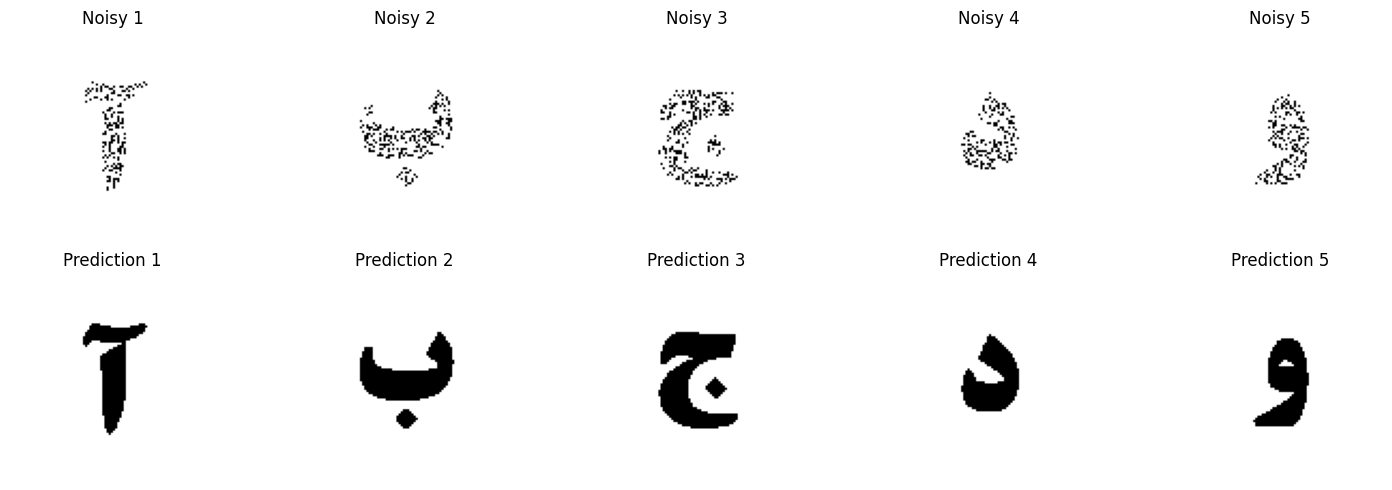
\includegraphics[width=\textwidth]{5.png}
    \caption{Top row: Missed images (70\% erasure). Bottom row: Predictions using masked Hamming network.}
    \label{fig:masked_hamming_output}
\end{figure}



\end{document}



